
\documentclass[a4paper,12pt]{article} % добавить leqno в [] для нумерации слева

\usepackage[left=2cm,right=2cm,
top=2cm,bottom=2cm,bindingoffset=0cm]{geometry}


\usepackage{cmap}

\usepackage{amsmath,amsfonts,amssymb,amsthm,mathtools} % AMS
\usepackage{mathtext}
\usepackage[TS1,T2A]{fontenc}
\usepackage[utf8]{inputenc}
\usepackage{siunitx}

\usepackage[english,russian]{babel}

\usepackage{fontspec}         % пакет для подгрузки шрифтов

\setmainfont{Times New Roman}       % задаёт основной шрифт документа


\usepackage{icomma} 
\mathtoolsset{showonlyrefs=true} % Показывать номера только у тех формул, на которые есть \eqref{} в тексте.
\usepackage{euscript}	 % Шрифт Евклид
\usepackage{mathrsfs} % Красивый матшрифт
\usepackage{enumitem}
\usepackage{tikz} % To generate the plot from csv
\usepackage{pgfplots}

\usepackage{multicol}
\setlength{\columnsep}{1cm}

%\renewcommand{\theenumi}{(\Asbuk{enumi})}
%\renewcommand{\labelenumi}{\Asbuk{enumi})}

\makeatletter
\AddEnumerateCounter{\asbuk}{\russian@alph}{щ}
\makeatother

%%% Заголовок
\author{Касьянова Ксения, Федорчук Яна (ЭО-15-01) }
\title{Домашнее задание 2}
\date{\today}


\begin{document}

\maketitle

\subsubsection*{(а)}	

Сравним средние уровни инфляции в таргетирующих её странах:  до инфляционного таргетирования $ \bar{X}_{pre} = 10.9 $ и после инфляционного таргетирования $ \bar{X}_{post} = 5.09$. 

Проведем парный t-тест: $ t = 3.355, p-value = 0.002294$

Значение $ p-value < 0.05 $ говорит о том, что разница в средних $ \Delta \bar{X} = 5.8 $  статистически значима.    
	
\begin{figure}[h!]
	\centering
	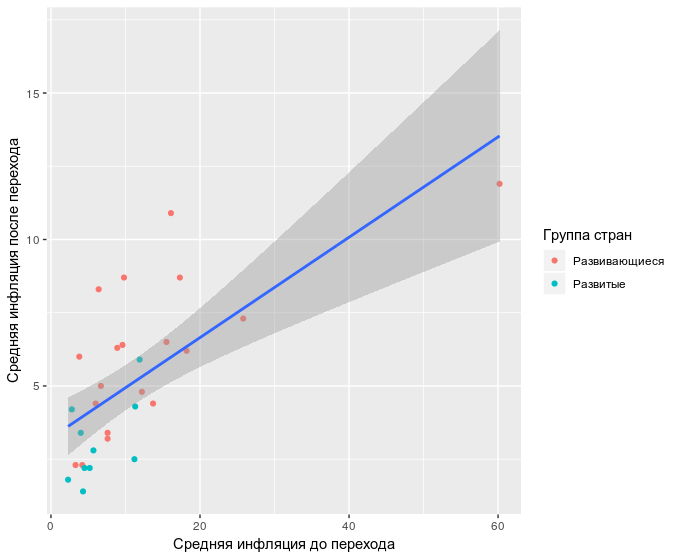
\includegraphics[width=0.7\linewidth]{Rplot}
	\caption[Диаграмма рассеяния]{Диаграмма рассеяния}
	\label{fig:rplot1}
\end{figure}


Можно ли на основе
этого результата сделать вывод о воздействии инфляционного
таргетирования на уровень инфляции?




	
	
\subsubsection*{(б)}	

Оценим регрессию разницы уровней инфляции до и после инфляционного таргетирования по дамми, которая равна 1, если страна таргетирует инфляцию.

\newpage

Для полной выборки стран:

\begin{table}[h!]
	\centering
	\begin{tabular}{rrrrr}
		\hline
		& Estimate & Std. Error & t value & Pr(>|t|) \\ 
		\hline
		(Intercept) & -0.2362 & 0.9807 & -0.24 & 0.8101 \\ 
		$ D $ & -5.5707 & 2.1081 & -2.64 & 0.0092 \\ 
		\hline
	\end{tabular}
\end{table}

,
Для выборки развивающихся стран:

\begin{table}[h!]
	\centering
	\begin{tabular}{rrrrr}
		\hline
		& Estimate & Std. Error & t value & Pr(>|t|) \\ 
		\hline
		(Intercept) & -2.2727 & 0.5766 & -3.94 & 0.0004 \\ 
		$ D $ & -0.9773 & 1.0315 & -0.95 & 0.3510 \\ 
		\hline
		\end{tabular}
		\end{table}

Для выборки развитых стран:

\begin{table}[h!]
	\centering
	\begin{tabular}{rrrrr}
		\hline
		& Estimate & Std. Error & t value & Pr(>|t|) \\ 
		\hline
		(Intercept) & 0.3036 & 1.2465 & 0.24 & 0.8081 \\ 
		$ D $ & -7.4562 & 2.8881 & -2.58 & 0.0113 \\ 
		\hline
		\end{tabular}
		\end{table}

Интерпретируйте полученные результаты: объясните, что можно
сказать о воздействии перехода к инфляционному таргетированию на
уровень инфляции в долгосрочной перспективе, опираясь на полученные
оценки параметров?

При добавлении latitude в качестве регрессора  
оценка коэффициента при индексе институтов prot практически не изменяется. Сама переменная статистически значима и имеет положительный знак.



\subsubsection*{(в)}	

Оценим регрессию разницы уровней инфляции до и после инфляционного таргетирования по дамми, которая равна 1, если страна таргетирует инфляцию, и контрольной перменной  $ X_pre $ значению инфляции до таргетирования.
 
Для полной выборки стран:
 
\begin{table}[h!]
	\centering
	\begin{tabular}{rrrrr}
		\hline
		& Estimate & Std. Error & t value & Pr(>|t|) \\ 
		\hline
		(Intercept) & 4.7618 & 0.3619 & 13.16 & 0.0000 \\ 
		$ D $ & -1.2539 & 0.7164 & -1.75 & 0.0824 \\ 
		$ X_pre $ & -0.8546 & 0.0263 & -32.45 & 0.0000 \\ 
		\hline
	\end{tabular}
\end{table}

Для выборки развивающихся стран:

\begin{table}[h!]
	\centering
	\begin{tabular}{rrrrr}
		\hline
		& Estimate & Std. Error & t value & Pr(>|t|) \\ 
		\hline
		(Intercept) & 0.8521 & 0.3672 & 2.32 & 0.0275 \\ 
		$ D $ & 0.3088 & 0.4574 & 0.68 & 0.5049 \\ 
		$ X_pre $ & -0.6979 & 0.0605 & -11.54 & 0.0000 \\ 
		\hline
	\end{tabular}
\end{table}

Для выборки развитых стран:

\begin{table}[h!]
	\centering
	\begin{tabular}{rrrrr}
		\hline
		& Estimate & Std. Error & t value & Pr(>|t|) \\ 
		\hline
		(Intercept) & 5.7226 & 0.4033 & 14.19 & 0.0000 \\ 
		$ D $ & -1.2640 & 0.8717 & -1.45 & 0.1502 \\ 
		$ X_pre $  & -0.8723 & 0.0269 & -32.46 & 0.0000 \\ 
		\hline
	\end{tabular}
\end{table}


Интерпретируйте полученные
результаты. Сопоставьте полученные оценки с результатами пункта (б).
Поясните причины отличий.

Сделайте вывод о влиянии инфляционного таргетирования на
уровень инфляции в развитых странах. Сделайте вывод о влиянии
инфляционного таргетирования на уровень инфляции в развивающихся
странах.


Оценка коэффициента при переменной смертности меньше нуля, что верно согласно аргументам, приведенным в статье,  и логике: чем выше смертность колонистов, тем ниже будет ВВП в колониях, т.е. поскольку колонии, где европейцы сталкиваются с более высокими показателями смертности, сегодня значительно беднее колоний, которые были здоровы для европейцев. 


\subsubsection*{(г)}	

Данный
инструмент можно  считать валидным, что 
позволяет корректно тестировать наличие причинно-следственной
связи между качеством институтов и ВВП, поскольку коэффициенты смертности европейских поселенцев более 100 лет назад не влияют на ВВП на душу населения сегодня, кроме их влияния за счет институционального развития. 
Также мы можем подтвердить, что наши результаты не обусловлены пропущенными факторами, т.е. нет других факторов, связанных с оценкой смертности поселенцев, влияющих на доход на душу населения: 
включение ряда переменных, которые потенциально коррелируют с летальностью поселенцев и экономическими результатами, не  отменяет наши результаты.
Невозможно контролировать все возможные переменные, которые могут быть коррелированы с летальностью поселенцев и экономическими результатами, а выбор нашего инструмента мог бы отразить влияние смертности поселенцев на экономические показатели через  другие каналы. Эти проблемы выявляются   с помощью  теста  Саргана.
 

\subsubsection*{(е)}	

Оценка влияния качества институтов на ВВП по
сравнению с оценкой выросла c $ \beta_{OLS} = 0.5221 $ до  $ \beta_{2SLS} = 0.9171 $. Такое
изменение говорит о наличии пропущенных переменных как причины эндогенности в первоначальной модели.


\subsubsection*{(ж)}

Сравним эффект воздействия качества институтов на ВВП на этой
подвыборке с оценками на базовой выборке. 
Мы подтверждаем, что оценки влияния институтов на эффективность не обусловлены выбросами, т.е. наши результаты  не изменяются при  исключении Африки. 

Данный эффект является гетерогенным, поскольку качество модели резко снижается при использовании подвыборки только с африканскими странами с $ multiple \ R^2_{without \ Africa} = 0.588   $ до $ multiple \ R^2_{with \ Africa} = -6.24  $  для первой модели и с $ multiple \ R^2_{without \ Africa} = 0.5894   $  до $ multiple \ R^2_{with \ Africa} = -14.11   $  для второй.   
	
\subsubsection*{(з)}	

Критик утверждает, что высокий ВВП на душу
населения 
объясняется прежде всего не качеством институтов, а высокой долей
населения европейского происхождения в общем населении этих стран.
Если критик прав и коэффициент при переменной euro будет значимой, то оценки в 2МНК уже не будут  состоятельными.
  


\subsubsection*{(и)}	

Проверим гипотезу, сформулированную критиком. 

Оценим регрессию логарифма ВВП по индексу институтов с помощью 2МНК, где инструментом является смертность  поселенцев, а контрольной переменной доля населения европейского происхождения в данной
стране.


Оценим альтернативную регрессию логарифма ВВП по индексу институтов с помощью 2МНК, где инструментом является смертность  поселенцев, а контрольными переменной - широта доля населения европейского происхождения в данной
стране.


В этих регрессиях ни расстояние от экватора, ни доля европейского населения не являются значимыми. Критик неправ. Эти результаты показывают, что некоторые страны  беднее других не из-за чистых географических или демографических  факторов, а из-за худших институтов.


	

\end{document}